\subsection{Closed objective-conditioned native search}
\label{sec:prescale-search}
The next study completes an objective-conditioned loop in the same original
researcher world, rather than a simplified numerical society. It uses an
unchanged executable source, \code{62388a7}, five fixed Qwen3-8B researchers,
four annual cycles and the existing local 35B designer. Before scientific
dispatch, its own two numerical and 28 staged-editor controls pass, including
cold replay. This is interface evidence, not a guarantee that free proposals
will execute. No post-hoc repair is applied to a received scientific proposal.

\paragraph{Finite comparison and fixed selection.}
There are two assigned losses, T and E, and four proposal methods: six literal
numerical coordinates, generated source with fixed wiring, generated source
and graph, and a uniform numerical comparator. Each arm consumes two proposal
slots on development seed 41001. Generated proposals can use their own prior
recorded result; the open-seed loss is included in final comparison but is
not exposed before the first proposal. Six separately executed references
include the open seed, legacy system, reviewed accept-all, no-review
accept-all, no-review reject-all and an information-disconnected system.
The production, calendar and accounting boundary is fixed for this pilot;
institutional algorithms, entities, memory and routes remain editable. This
is an explicit comparison domain, not an outcome veto or the global design
ceiling. C is evaluated only as a diagnostic and does not select a proposal.

All 16 slots are consumed: 11 complete and five fail during execution, with
no generation failures, replacement slots or imputed losses.
Table~\ref{tab:prescale-slots} retains every slot; Figure~\ref{fig:prescale-paths}
shows best-so-far paths including the common initial comparison. Selection
freezes at 07:47:45 UTC on November 9, before evaluation starts at 07:47:57.
Within each arm, the lowest available own loss wins, including the initial
system; exact ties retain the earliest declared row. Three previously unused
seeds (51001, 51011, 51017) then evaluate each selected policy and four
references. Twelve labels times three seeds give 36 logical rows but only
27 physical jobs, because exactly identical policies share execution.
All 27 complete at 11:29:22 UTC. Two full original-source audits subsequently
match byte for byte, covering 1,859 raw files and all 49 physical worlds:
six development references, 16 submitted candidates and 27 evaluations.
Five of the 49 are the retained partial runtime failures, not completed worlds.

\begin{table}[htbp]
\centering\small
\caption{All 16 development slots. Entries are assigned proxy losses, lower
is better; F denotes a runtime failure with unavailable loss. Selection also
includes the common initial (T: 0, E: 43.5), hence an initial can win.}
\label{tab:prescale-slots}
\begin{tabular}{llrrl}
\toprule Objective & Method & G0 & G1 & Fixed selection\\
\midrule
T & Numerical & $-14$ & $-14$ & G0 (earliest tie)\\
T & Code / fixed graph & $-14$ & F & G0\\
T & Code and graph & F & F & Initial\\
T & Uniform & $0$ & $-2$ & G1\\
E & Numerical & $29.333$ & $-22.667$ & G1\\
E & Code / fixed graph & F & F & Initial\\
E & Code and graph & $27$ & $43.5$ & G0\\
E & Uniform & $43.5$ & $34.667$ & G1\\
\bottomrule
\end{tabular}
\end{table}

\begin{figure}[htbp]
\centering
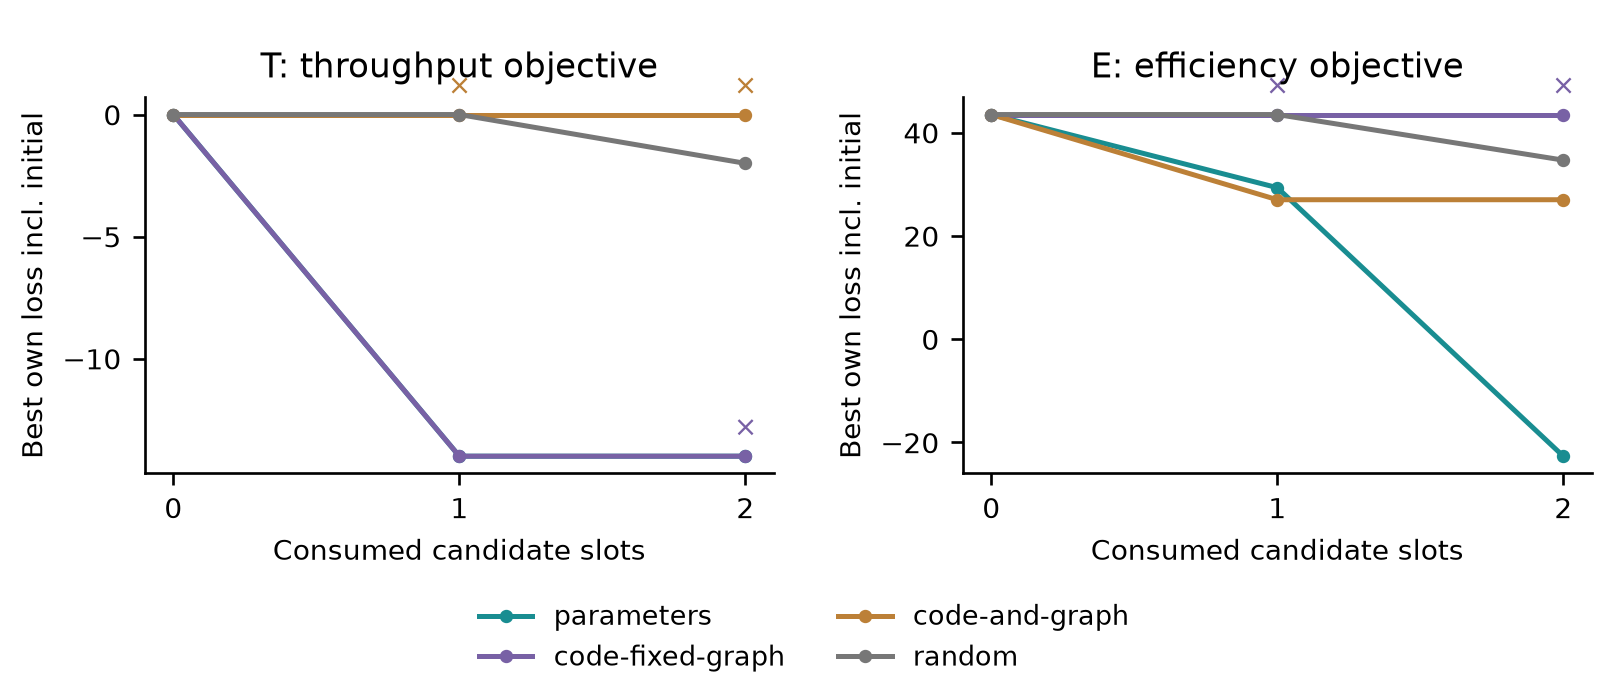
\includegraphics[width=\linewidth]{figures/pre-scale-search-v1/objective-conditioned-paths.png}
\caption{Actual two-slot optimization paths, not additional simulations or
fitted response surfaces. Slot 0 is the common initial included for final
comparison; subsequent points are the best eligible loss including it. Crosses
mark consumed failed slots and do not assign those proposals a loss. The T
numerical and fixed-graph code paths coincide exactly. The E numerical G1
decrease is an observed development result, not established optimizer superiority.}
\label{fig:prescale-paths}
\end{figure}

\paragraph{What the optimizer actually changes.}
E/numerical G0 has A=2, Q=$6\frac{2}{3}$ and R=72, hence E=$29\frac{1}{3}$.
The next request contains that observed loss. Its submitted G1 changes the
memory-router threshold from 1 to 0 while retaining the other five literal
coordinates; A=14, Q=$43\frac{2}{3}$ and R=42 give E=$-22\frac{2}{3}$.
The router's actual native consumer is operative: the G0 rule can reject
after its accumulated-memory penalty, whereas G1 accepts at the changed
threshold. This establishes an executed feedback-history update, not that
the author's explanation is correct or that feedback caused the improvement
relative to another search method.

Free-source proposals do not simply select from built-in rules. The completed
T/fixed-graph G0 writes an always-accept decision rule; E/code-and-graph G0
writes always-reject with a literal zero final score; its G1 uses the original
review-score average with a threshold above 5 and changes addressed thresholds
and bias. Those free-code values need not lie in the six-coordinate numerical
box. Nevertheless, all 16 submissions retain the initial 21 mechanisms,
29 connections and schedules: eight change source, none changes literal
wiring or scheduling. Allowed structural freedom therefore does not establish
realized topology invention. Rejecting after review does not itself avoid the
earlier review operation, contrary to one generated comment; source rationale
is not a validated mechanism explanation.

The five failures are substantive execution records: an unwrapped world
payload, missing decision fields, \code{score} instead of
\code{final\_score}, a float treated as a sequence, and incomplete submitted-paper
identity coverage. Readiness did not prevent these free-design mistakes.
They remain unavailable-loss outcomes and consume their declared slots.
A separate later output-envelope advisory is tested but is not backported
into this experiment, and it does not automatically repair generated source.

\paragraph{Selection-fixed common evaluation.}
Table~\ref{tab:prescale-evaluation} and Figure~\ref{fig:prescale-common}
report all selected labels and four references under the same three losses.
The E/numerical policy averages $-17.333$ on E versus $-16.889$ for reviewed
accept-all, a paired mean difference of $-4/9$. The three differences are
$-1,-2/3,+1/3$: the sign varies, and this small study does not establish
superiority. Their accepted counts and review counts match; the difference
is in endogenous review-score sums, not verified scientific value or an
isolated causal information effect. T/numerical, T/fixed-graph and reviewed
accept-all have identical observed score vectors but different literal
policies and separately executed jobs. By contrast, the two selected uniform
labels really do share jobs; the initial reference is also shared with the
selected E/fixed-graph and T/code-and-graph labels. Neither equal outcomes
nor duplicate labels create independent evidence.

\begin{table}[htbp]
\centering\small
\caption{All selection-fixed labels: three-seed means of native components
and common losses (all 3/3 available). A counts accepted decisions; Q sums
endogenous accepted peer scores; R counts review records. Q=0 without review
is a measurement convention, not evidence of zero scientific quality.}
\label{tab:prescale-evaluation}
\begin{tabular}{lrrrrrr}
\toprule Label & A & Q & R & T & E & C\\
\midrule
Ref: open seed & 0 & 0 & 67 & 0 & 33.500 & 6.700\\
Ref: reviewed accept-all & 10.667 & 32.889 & 32 & $-10.667$ & $-16.889$ & 12.978\\
Ref: no-review accept-all & 10.667 & 0 & 0 & $-10.667$ & 0 & 42.667\\
Ref: no-review reject-all & 0 & 0 & 0 & 0 & 0 & 0\\
\midrule
T: numerical & 10.667 & 32.889 & 32 & $-10.667$ & $-16.889$ & 12.978\\
T: code / fixed graph & 10.667 & 32.889 & 32 & $-10.667$ & $-16.889$ & 12.978\\
T: code and graph & 0 & 0 & 67 & 0 & 33.500 & 6.700\\
T: uniform & 1.667 & 6.111 & 61 & $-1.667$ & 24.389 & 6.656\\
E: numerical & 10.667 & 33.333 & 32 & $-10.667$ & $-17.333$ & 12.533\\
E: code / fixed graph & 0 & 0 & 67 & 0 & 33.500 & 6.700\\
E: code and graph & 0 & 0 & 35 & 0 & 17.500 & 3.500\\
E: uniform & 1.667 & 6.111 & 61 & $-1.667$ & 24.389 & 6.656\\
\bottomrule
\end{tabular}
\end{table}

\begin{figure}[htbp]
\centering
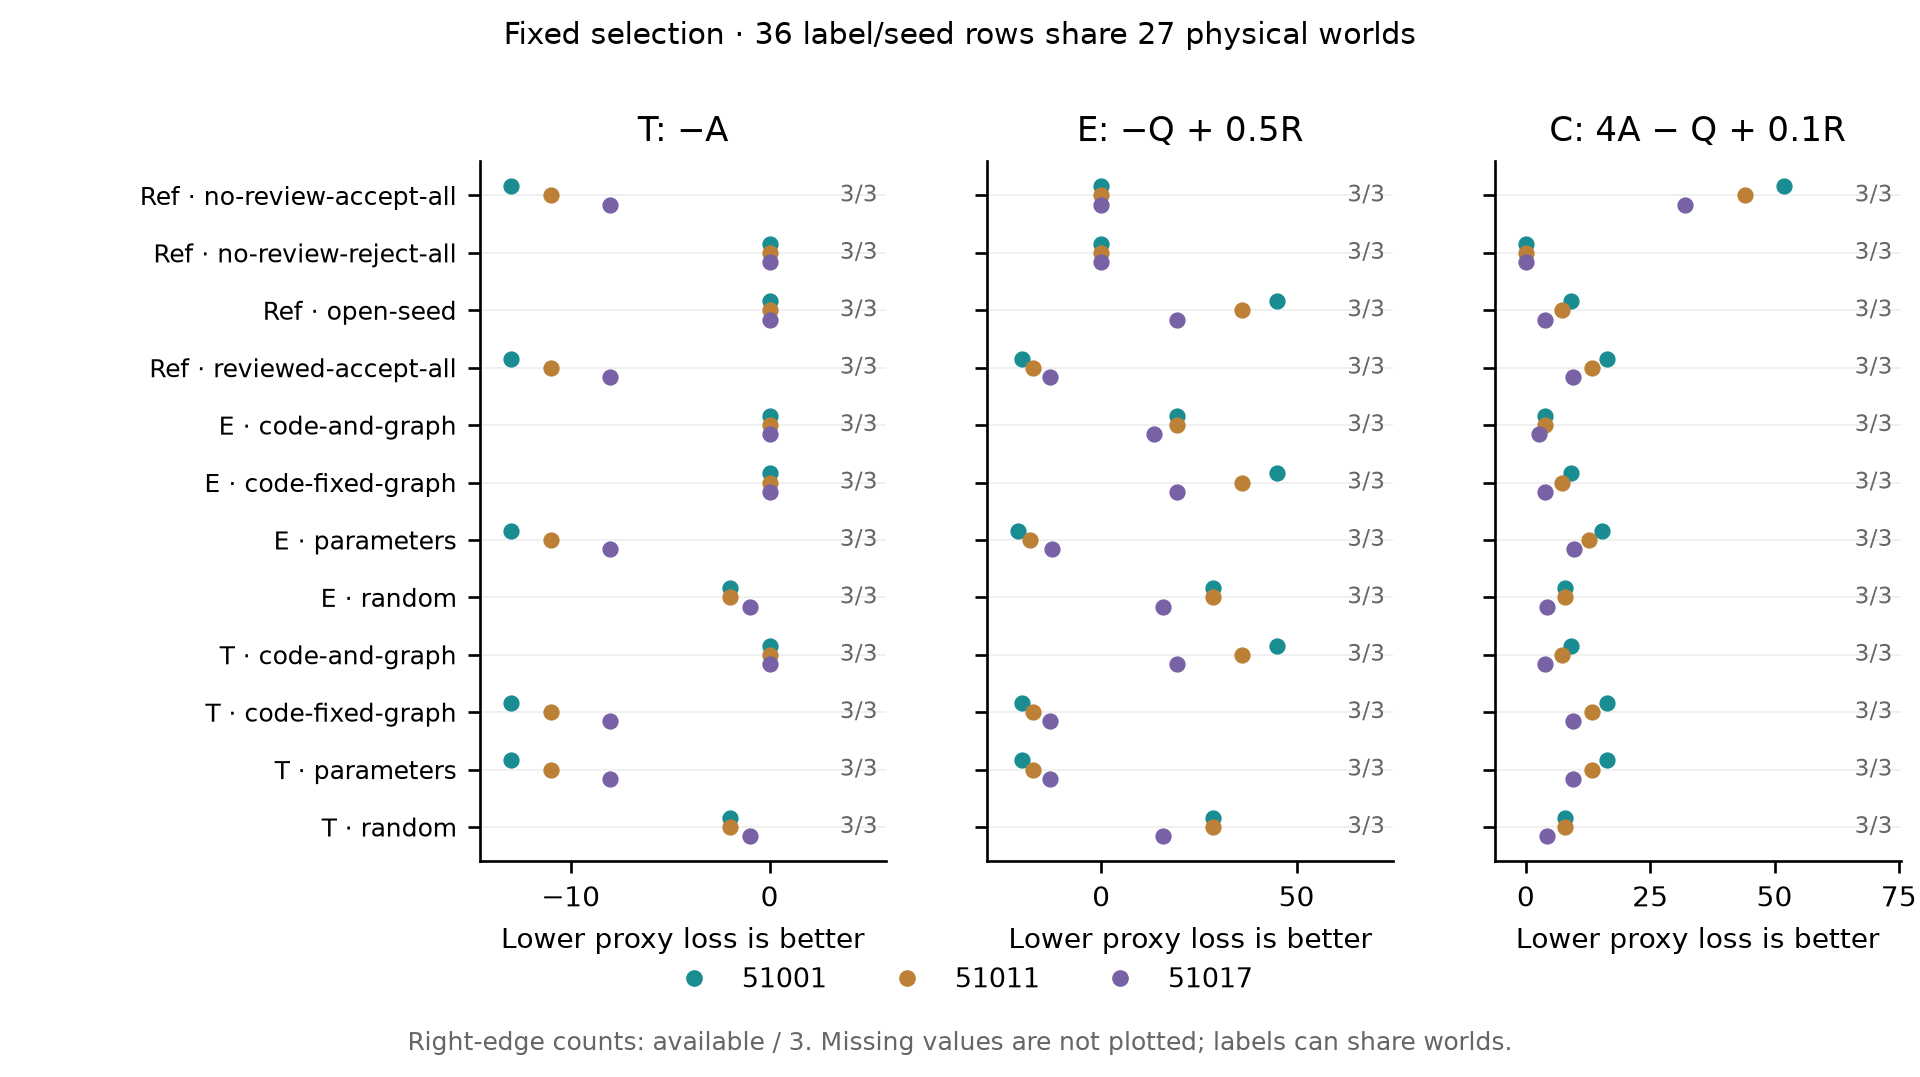
\includegraphics[width=\linewidth]{figures/pre-scale-search-v1/selection-fixed-common-scores.png}
\caption{Every selection-fixed seed score under T, E and diagnostic C. Colors
identify seeds, not independent repeats of shared policies. The right-edge
counts retain score availability. Strong reference rules expose proxy geometry:
unreviewed acceptance has no recorded Q or R, whereas reviewed acceptance can
make E negative. C was not searched in this pilot; its apparent reference
ordering is not an optimized-C result.}
\label{fig:prescale-common}
\end{figure}

\paragraph{Measured components, costs and reproducibility.}
Across the 49 physical forwards, scientist journals contain 8,025 completed
responses, 8,453,441 reported input and 723,376 output tokens; 1,416,327 cached
prompt tokens are a subset of input, not additional work. All five partial
failures retain their charged replies. Designer proposal records include six
numerical calls (25,651 input, 8,461 output tokens) and 104 staged-editor calls
(2,076,602 input, 39,372 output tokens). Readiness is separate: three numerical
calls and 28 editor controls. Numeric caller intervals total 201.790 seconds;
editor transport intervals total 1,533.432 seconds, and role loads are kept
separate. These component counters and overlapping timing aliases are not
added into project FLOPs, energy, money or total compute. The scientific search
and evaluation stages occupy about 7 hours 18 minutes end to end on this local
binding, excluding earlier readiness, audits and all software-development work.

Retained data contain every executable submitted system, physical-world join,
raw component status, exact selection tie, shared-job identity and 96 paired
reference comparisons. Independent numerical rebuilding recomputes their
cross-scores and regenerates both figures byte-identically; a separate literal
change projection records actual source/interface/wiring differences. Full
raw/source auditing, retained-data numerical rebuilding and fresh inference
remain different reproducibility levels. The English Foundry now inspects
this closed study's actual development code, ports, connections, year snapshots
and failures; it neither turns development records into unused-seed evidence
nor submits another simulation.
